\documentclass[authordate, empirical]{jote-new-article}



\addbibresource{bibliography.bib}

\begin{filecontents}{bibliography.bib}

  @article{Blass2006,
  title       = {On the road to obesity: Television viewing increases intake of high-density foods},
  author      = {Blass, E. M. and Anderson, D. R. and Kirkorian, H. L. and Pempek, T. A. and Price, I. and Koleini, M. F.},
  number      = {4-5},
  volume      = {88},
  url         = {https://doi.org/10.1016/j.physbeh.2006.05.035},
  doi         = {10.1016/j.physbeh.2006.05.035},
  publisher   = {Elsevier BV},
  date        = {2006},
  pages       = {597-604},
  journal     = {Physiology \& Behavior}
}



@article{Boon2002,
        doi = {10.1348/135910702169303},
        url = {https://doi.org/10.1348/135910702169303},
        year = 2002,
        month = {feb},
        publisher = {Wiley},
        volume = {7},
        number = {1},
        pages = {1--10},
        author = {Brigitte Boon and Wolfgang Stroebe and Henk Schut and Richta Ijntema},
        title = {Ironic processes in the eating behaviour of restrained eaters},
        journal = {British Journal of Health Psychology}
}




@article{Forde2018,
    title       = {From perception to ingestion: The role of sensory properties in energy selection, eating behaviour and food intake.},
    journal     = {Food Quality and Preference},
    volume      = {66},
    author      = {Forde, C. G.},
    date        = {2018},
    pages       = {171–177}
}





@article{Higgs2009,
    title       = {Television watching during lunch increases afternoon snack intake of young women},
    author      = {Higgs, S. and Woodward, M.},
    journal     = {Appetite},
    volume      = {52},
    date        = {2009},
    pages       = {39–43}
}


@article{Hirschberg2016,
    title       = {The changing market for food delivery},
    author      = {Hirschberg, C. and Rajko, A. and Schumacher, T. and Wrulich, M.},
    url         = {https://www.mckinsey.com/industries/technology-media-and-telecommunications/our-insights/the-changing-market-for-food-delivery},
    date        = {2016-11-09},
    journal     = {Mckinsey and Co}
}



@article{RCoreTeam2019,
    title       = {R: A language and environment for statistical computing. {R Foundation for Statistical Computing}},
    author      = {{R Core Team}},
    url         = {https://www.R-project.org/.},
    date        = {2019}
}


@article{Reichenberger2018,
    title       = {No haste, more taste: An {EMA} study of the effects of stress, negative and positive emotions on eating behavior },
    author      = {Reichenberger, J. and Kuppens, P. and Liedlgruber, M. and Wilhelm, F. H. and Tiefengrabner, M. and Ginzinger, S. and Blechert, J.},
    date        = {2018},
    pages       = {54–62},
    journal     = {Biological Psychology},
    volume      = {131}
}






@article{Small2019,
    author      = {Small, D. M. and DiFeliceantonio, A. G.},
    number      = {6425},
    volume      = {363},
    date        = {2019},
    pages       = {346–347},
    title = {Processed foods and food rewards},
    journal = {Science}
}





@article{Tang2014,
    title       = {Behavioral and neural valuation of foods is driven by implicit knowledge of caloric content. },
    author      = {Tang, D. W. and Fellows, L. K. and Dagher, A.},
    date        = {2014},
    journal     = {Psychological Science},
    volume      = {25},
    number      = {12},
    pages       = {2168–2176}
}

@article{Tobin1958,
        doi = {10.2307/2296205},
        url = {https://doi.org/10.2307/2296205},
        year = 1958,
        month = {feb},
        publisher = {Oxford University Press ({OUP})},
        volume = {25},
        number = {2},
        pages = {65},
        author = {J. Tobin},
        title = {Liquidity Preference as Behavior Towards Risk},
        journal = {The Review of Economic Studies}
}          



@article{VoedingscentrumND,
    title       = {Wat is de voedingswaarde van chips op basis van aardappelmeel},
    author      = {{Voedingscentrum}},
    url         = {https://www.voedingscentrum.nl/nl/service/vraag-en-antwoord/gezonde-voeding-en-voedingsstoffen/hoeveel-voedingswaarden-zitten-erin/chips-op-basis-van-aardappelmeel.aspx},
    date        = {n.d.}
}




@article{Antoun2017,
title       = {The acute physiological stress response to driving: A systematic review},
author      = {Antoun, Michael and Edwards, Kate M. and Sweeting, Joanna and Ding, Ding},
editor      = {Xu, Jun},
number      = {10},
volume      = {12},
url         = {https://doi.org/10.1371/journal.pone.0185517},
doi         = {10.1371/journal.pone.0185517},
publisher   = {Public Library of Science (PLoS)},
date        = {2017-10-16},
pages       = {e0185517},
journal     = {PLOS ONE}
}



@article{Bolhuis2012,
title       = {Effect of salt intensity in soup on ad libitum intake and on subsequent food choice},
author      = {Bolhuis, Dieuwerke P. and Lakemond, Catriona M.M. and de Wijk, Rene A. and Luning, Pieternel A. and de Graaf, Cees},
number      = {1},
volume      = {58},
url         = {https://doi.org/10.1016/j.appet.2011.09.001},
doi         = {10.1016/j.appet.2011.09.001},
publisher   = {Elsevier BV},
date        = {2012-02},
pages       = {48-55},
journal     = {Appetite}
}


@article{Crespo2001,
        doi = {10.1001/archpedi.155.3.360},
        url = {https://doi.org/10.1001/archpedi.155.3.360},
        year = 2001,
        month = {mar},
        publisher = {American Medical Association ({AMA})},
        volume = {155},
        number = {3},
        pages = {360},
        author = {Carlos J. Crespo and Ellen Smit and Richard P. Troiano and Susan J. Bartlett and Caroline A. Macera and Ross E. Andersen},
        title = {Television Watching, Energy Intake, and Obesity in {US} Children},
        journal = {Archives of Pediatrics \& Adolescent Medicine}
}


@article{DiFeliceantonio2018,
title       = {Supra-additive effects of combining fat and carbohydrate on food reward},
journal      = { Cell Metabolism},
volume      = {28},
number      = {1},
author      = {DiFeliceantonio, A. G. and Coppin, G. and Rigoux, L. and Thanarajah, S. E. and Dagher, A. and Tittgemeyer, M. and Small, D. M.},
date        = {2018},
pages       = {33–44}
}


@article{Dingus2016,
title       = {Driver crash risk factors and prevalence evaluation using naturalistic driving data},
author      = {Dingus, Thomas A. and Guo, Feng and Lee, Suzie and Antin, Jonathan F. and Perez, Miguel and Buchanan-King, Mindy and Hankey, Jonathan},
number      = {10},
volume      = {113},
url         = {https://doi.org/10.1073/pnas.1513271113},
doi         = {10.1073/pnas.1513271113},
publisher   = {Proceedings of the National Academy of Sciences},
date        = {2016-02-22},
pages       = {2636-2641},
journal     = {Proceedings of the National Academy of Sciences}
}


@article{Dubois2008,
title       = {Social factors and television use during meals and snacks is associated with higher BMI among pre-school children},
author      = {Dubois, Lise and Farmer, Anna and Girard, Manon and Peterson, Kelly},
number      = {12},
volume      = {11},
url         = {https://doi.org/10.1017/s1368980008002887},
doi         = {10.1017/s1368980008002887},
publisher   = {Cambridge University Press (CUP)},
date        = {2008-12},
pages       = {1267-1279},
journal     = {Public Health Nutrition}
}


@article{Duif2020,
title       = {Effects of distraction on taste-related neural processing: a cross-sectional {fMRI} study},
author      = {Duif, Iris and Wegman, Joost and Mars, Monica M and de Graaf, Cees and Smeets, Paul AM and Aarts, Esther},
number      = {5},
volume      = {111},
url         = {https://doi.org/10.1093/ajcn/nqaa032},
doi         = {10.1093/ajcn/nqaa032},
publisher   = {Elsevier BV},
date        = {2020-05},
pages       = {950-961},
journal     = {The American Journal of Clinical Nutrition}
}


@inbook{Monitor2018,
title       = {{FSIN FoodShopper Monitor 2019}},
author      = {{FoodShopper Monitor}},
url         = {https://fsin.nl/foodshoppermonitor},
date        = {2018},
booktitle     = {FoodService Instituut Nederland}
}





@article{Forde2013,
title       = {Oral processing characteristics of solid savoury meal components, and relationship with food composition, sensory attributes and expected satiation},
author      = {Forde, C. G. and van Kuijk, N. and Thaler, T. and de Graaf, C. and Martin, N.},
volume      = {60},
url         = {https://doi.org/10.1016/j.appet.2012.09.015},
doi         = {10.1016/j.appet.2012.09.015},
publisher   = {Elsevier BV},
date        = {2013-01},
pages       = {208-219},
journal     = {Appetite}
}


@article{Henningsen2010,
title       = {Estimating censored regression models in {R using the censReg Package}},
author      = {Henningsen, A.},
volume      = {5},
date        = {2010},
pages       = {1–12},
journal     = {R Package Vignettes}
}


@article{Hoffmann-Hensel2017,
title       = {Cognitive Load Alters Neuronal Processing of Food Odors},
author      = {Hoffmann-Hensel, Sonja Maria and Sijben, Rik and Rodriguez-Raecke, Rea and Freiherr, Jessica},
number      = {9},
volume      = {42},
url         = {https://doi.org/10.1093/chemse/bjx046},
doi         = {10.1093/chemse/bjx046},
publisher   = {Oxford University Press (OUP)},
date        = {2017-08-10},
pages       = {723-736},
journal     = {Chemical Senses}
}


@article{Higgs2011,
title       = {Focusing on food during lunch enhances lunch memory and decreases later snack intake},
author      = {Higgs, Suzanne and Donohoe, Jessica E.},
number      = {1},
volume      = {57},
url         = {https://doi.org/10.1016/j.appet.2011.04.016},
doi         = {10.1016/j.appet.2011.04.016},
publisher   = {Elsevier BV},
date        = {2011-08},
pages       = {202-206},
journal     = {Appetite}
}


@article{Higgs2008,
title       = {Recall of recent lunch and its effect on subsequent snack intake},
author      = {Higgs, Suzanne and Williamson, Amy C. and Attwood, Angela S.},
number      = {3},
volume      = {94},
url         = {https://doi.org/10.1016/j.physbeh.2008.02.011},
doi         = {10.1016/j.physbeh.2008.02.011},
publisher   = {Elsevier BV},
date        = {2008-06},
pages       = {454-462},
journal     = {Physiology \& Behavior}
}





@article{Irwin2015,
title       = {The Influence of Drinking, Texting, and Eating on Simulated Driving Performance},
author      = {Irwin, Christopher and Monement, Sophie and Desbrow, Ben},
number      = {2},
volume      = {16},
url         = {https://doi.org/10.1080/15389588.2014.920953},
doi         = {10.1080/15389588.2014.920953},
publisher   = {Informa UK Limited},
date        = {2014-10-15},
pages       = {116-123},
journal     = {Traffic Injury Prevention}
}


@article{Liang2018,
title       = {Memory Load Influences Taste Sensitivities},
author      = {Liang, Pei and Jiang, Jiayu and Ding, Qingguo and Tang, Xiaoyan and Roy, Soumyajit},
volume      = {9},
url         = {https://doi.org/10.3389/fpsyg.2018.02533},
doi         = {10.3389/fpsyg.2018.02533},
publisher   = {Frontiers Media SA},
date        = {2018-12-11},
journal     = {Frontiers in Psychology}
}


@article{McCrickerd2016,
title       = {Sensory influences on food intake control: moving beyond palatability},
author      = {McCrickerd, K. and Forde, C. G.},
number      = {1},
volume      = {17},
url         = {https://doi.org/10.1111/obr.12340},
doi         = {10.1111/obr.12340},
publisher   = {Wiley},
date        = {2015-12-11},
pages       = {18-29},
journal     = {Obesity Reviews}
}


@article{Morris2020,
title       = {Ingested but not perceived: Response to satiety cues disrupted by perceptual load},
author      = {Morris, Jenny and Vi, Chi Thanh and Obrist, Marianna and Forster, Sophie and Yeomans, Martin R.},
volume      = {155},
url         = {https://doi.org/10.1016/j.appet.2020.104813},
doi         = {10.1016/j.appet.2020.104813},
publisher   = {Elsevier BV},
date        = {2020-12},
pages       = {104813},
journal     = {Appetite}
}


@article{Moskowitz1972,
title       = {Perceptual changes in taste mixtures},
author      = {Moskowitz, Howard R.},
number      = {4},
volume      = {11},
url         = {https://doi.org/10.3758/bf03210374},
doi         = {10.3758/bf03210374},
publisher   = {Springer Science and Business Media LLC},
date        = {1972-07},
pages       = {257-262},
journal     = {Perception \& Psychophysics}
}


@article{Ogden2013,
title       = {Distraction, restrained eating and disinhibition: An experimental study of food intake and the impact of ‘eating on the go’},
author      = {Ogden, Jane and Oikonomou, Eirini and Alemany, Georgina},
number      = {1},
volume      = {22},
url         = {https://doi.org/10.1177/1359105315595119},
doi         = {10.1177/1359105315595119},
publisher   = {SAGE Publications},
date        = {2016-07-10},
pages       = {39-50},
journal     = {Journal of Health Psychology}
}


@article{Oldham-Cooper2010,
title       = {Playing a computer game during lunch affects fullness, memory for lunch, and later snack intake},
author      = {Oldham-Cooper, Rose E and Hardman, Charlotte A and Nicoll, Charlotte E and Rogers, Peter J and Brunstrom, Jeffrey M},
number      = {2},
volume      = {93},
url         = {https://doi.org/10.3945/ajcn.110.004580},
doi         = {10.3945/ajcn.110.004580},
date        = {2011-02},
pages       = {308-313},
journal     = {The American Journal of Clinical Nutrition}
}


@article{Polivy1978,
title       = {Internal and external components of emotionality in restrained and unrestrained eaters.},
author      = {Polivy, Janet and Herman, C. Peter and Warsh, Shelley},
number      = {5},
volume      = {87},
url         = {https://doi.org/10.1037/0021-843x.87.5.497},
doi         = {10.1037/0021-843x.87.5.497},
publisher   = {American Psychological Association (APA)},
date        = {1978-10},
pages       = {497-504},
journal     = {Journal of Abnormal Psychology}
}






@article{Robinson2013,
title       = {Eating attentively: a systematic review and meta-analysis of the effect of food intake memory and awareness on eating},
author      = {Robinson, Eric and Aveyard, Paul and Daley, Amanda and Jolly, Kate and Lewis, Amanda and Lycett, Deborah and Higgs, Suzanne},
number      = {4},
volume      = {97},
url         = {https://doi.org/10.3945/ajcn.112.045245},
doi         = {10.3945/ajcn.112.045245},
publisher   = {Elsevier BV},
date        = {2013-04},
pages       = {728-742},
journal     = {The American Journal of Clinical Nutrition}
}


@article{Robinson2014,
title       = {Eating ‘attentively’ reduces later energy consumption in overweight and obese females},
author      = {Robinson, Eric and Kersbergen, Inge and Higgs, Suzanne},
number      = {4},
volume      = {112},
url         = {https://doi.org/10.1017/s000711451400141x},
doi         = {10.1017/s000711451400141x},
publisher   = {Cambridge University Press (CUP)},
date        = {2014-06-16},
pages       = {657-661},
journal     = {British Journal of Nutrition}
}


@article{Rolls2008,
title       = {The orbitofrontal cortex and beyond: From affect to decision-making},
author      = {Rolls, Edmund T. and Grabenhorst, Fabian},
number      = {3},
volume      = {86},
url         = {https://doi.org/10.1016/j.pneurobio.2008.09.001},
doi         = {10.1016/j.pneurobio.2008.09.001},
publisher   = {Elsevier BV},
date        = {2008-11},
pages       = {216-244},
journal     = {Progress in Neurobiology}
}


@article{Rosseel2012,
title       = {lavaan: An {R} Package for Structural Equation Modeling},
author      = {Rosseel, Yves},
number      = {2},
volume      = {48},
url         = {https://doi.org/10.18637/jss.v048.i02},
doi         = {10.18637/jss.v048.i02},
publisher   = {Foundation for Open Access Statistic},
date        = {2012},
pages       = {1–36},
journal     = {Journal of Statistical Software}
}


@inbook{Rousseeuw2006,
title       = {A conceptual model of the food choice process over the life course.},
author      = {Sobal, J. and Bisogni, C. A. and Devine, C. M. and Jastran, M.},
volume      = {3},
url         = {https://doi.org/10.1079/9780851990323.0001},
doi         = {10.1079/9780851990323.0001},
publisher   = {CABI},
place       = {UK},
date        = {2006-01},
pages       = {1-18},
booktitle     = {The psychology of food choice}
}


@article{Spence2010,
title       = {The Influence of auditory cues on the perception of, and responses to, food and drink},
author      = {Spence, Charles and Shankar, Maya U.},
number      = {3},
volume      = {25},
url         = {https://doi.org/10.1111/j.1745-459x.2009.00267.x},
doi         = {10.1111/j.1745-459x.2009.00267.x},
publisher   = {Wiley},
date        = {2010-03-19},
pages       = {406-430},
journal     = {Journal of Sensory Studies}
}


@article{Stafford2013,
title       = {Music increases alcohol consumption rate in young females.},
author      = {Stafford, Lorenzo D. and Dodd, Hannah},
number      = {5},
volume      = {21},
url         = {https://doi.org/10.1037/a0034020},
doi         = {10.1037/a0034020},
publisher   = {American Psychological Association (APA)},
date        = {2013-10},
pages       = {408-415},
journal     = {Experimental and Clinical Psychopharmacology}
}


@article{Stroebele2006,
title       = {Listening to music while eating is related to increases in people's food intake and meal duration},
author      = {Stroebele, Nanette and de Castro, John M.},
number      = {3},
volume      = {47},
url         = {https://doi.org/10.1016/j.appet.2006.04.001},
doi         = {10.1016/j.appet.2006.04.001},
publisher   = {Elsevier BV},
date        = {2006-11},
pages       = {285-289},
journal     = {Appetite}
}


@article{Stutts2005,
title       = {Driver's exposure to distractions in their natural driving environment},
author      = {Stutts, Jane and Feaganes, John and Reinfurt, Donald and Rodgman, Eric and Hamlett, Charles and Gish, Kenneth and Staplin, Loren},
number      = {6},
volume      = {37},
url         = {https://doi.org/10.1016/j.aap.2005.06.007},
doi         = {10.1016/j.aap.2005.06.007},
publisher   = {Elsevier BV},
date        = {2005-11},
pages       = {1093-1101},
journal     = {Accident Analysis \& Prevention}
}



@article{Torres2007,
title       = {Relationship between stress, eating behavior, and obesity},
author      = {Torres, Susan J. and Nowson, Caryl A.},
number      = {11-12},
volume      = {23},
url         = {https://doi.org/10.1016/j.nut.2007.08.008},
doi         = {10.1016/j.nut.2007.08.008},
publisher   = {Elsevier BV},
date        = {2007-11},
pages       = {887-894},
journal     = {Nutrition}
}


@article{Wal2013,
title       = {Leaving a Flat Taste in Your Mouth},
author      = {van der Wal, Reine C. and van Dillen, Lotte F.},
number      = {7},
volume      = {24},
url         = {https://doi.org/10.1177/0956797612471953},
doi         = {10.1177/0956797612471953},
publisher   = {SAGE Publications},
date        = {2013-05-30},
pages       = {1277-1284},
journal     = {Psychological Science}
}

@article{Wallis2009,
title       = {Emotions and eating. {S}elf-reported and experimentally induced changes in food intake under stress},
journal     = {Appetite},
author      = {Wallis, D. J. and Hetherington, M. M.},
number      = {2},
volume      = {52},
date        = {2009},
pages       = {355–362}
}


@article{Wallis2004,
title       = {Stress and eating: the effects of ego-threat and cognitive demand on food intake in restrained and emotional eaters},
author      = {Wallis, D. J. and Hetherington, M. M.},
number      = {1},
volume      = {43},
url         = {https://doi.org/10.1016/j.appet.2004.02.001},
doi         = {10.1016/j.appet.2004.02.001},
publisher   = {Elsevier BV},
date        = {2004-08},
pages       = {39-46},
journal     = {Appetite}
}


@book{Yamauchi2013,
title       = {Gran Turismo [video game]},
author      = {Yamauchi, K.},
publisher   = {Sony Interactive Entertainment},
date        = {2013}
}


@article{Young2008,
title       = {Crash dieting: The effects of eating and drinking on driving performance},
author      = {Young, Mark S. and Mahfoud, Janina M. and Walker, Guy H. and Jenkins, Daniel P. and Stanton, Neville A.},
number      = {1},
volume      = {40},
url         = {https://doi.org/10.1016/j.aap.2007.04.012},
doi         = {10.1016/j.aap.2007.04.012},
publisher   = {Elsevier BV},
date        = {2008-01},
pages       = {142-148},
journal     = {Accident Analysis \& Prevention}
}


@article{Zontone2020,
title       = {Stress Evaluation in Simulated Autonomous and Manual Driving through the Analysis of Skin Potential Response and Electrocardiogram Signals},
author      = {Zontone, Pamela and Affanni, Antonio and Bernardini, Riccardo and Del Linz, Leonida and Piras, Alessandro and Rinaldo, Roberto},
number      = {9},
volume      = {20},
url         = {https://doi.org/10.3390/s20092494},
doi         = {10.3390/s20092494},
publisher   = {MDPI AG},
date        = {2020-04-28},
pages       = {2494},
journal     = {Sensors}
}
\end{filecontents}


\jotetitle{Driven to Snack: Simulated Driving Increases Subsequent Consumption}
\keywordsabstract{distracted eating, distraction, food intake, taste perception, consumption}
\abstracttext{When individuals eat while distracted, they may compensate by consuming more afterwards. Here, we examined the effect of eating while driving, and explored potential underlying mechanisms. Participants (\emph{N} = 116, 73.3\% female) were randomly allocated to complete a driving simulation (distraction condition) or to watch someone else drive (control condition) while consuming 10g (50.8 kcal) of potato chips. Afterwards, participants rated the taste intensity and hedonic experience, reported stress levels, and were then given the opportunity to eat more chips. As hypothesized, participants consumed more chips after the driving simulation. Stress levels were higher in the driving compared to control condition, but were inversely related to consumption amount, ruling out stress as explanatory mechanism. Saltiness ratings differed between the driving and passive viewing condition, only when controlling for stress. The current findings converge with earlier work showing that distracted eating can drive overconsumption, which in turn can lead to long-term health implications. Limitations, implications, and potential directions are discussed.}
\runningauthor{van Meer et al.}
\corremail{\href{mailto:a.f.van.meer@leidenuniv.nl}{a.f.van.meer@leidenuniv.nl}}
\corraddress{Social, Economic and Organizational Psychology Unit, Leiden University, P.O. Box 9555, 2300 RB Leiden, the Netherlands}
\jname{Journal of Trial \& Error}
\paperdoi{10.36850/e13}
\paperreceived{November 12, 2022}
\paperaccepted{March 21, 2023}
\jwebsite{https://journal.trialanderror.org}
\jyear{2023}
\paperpublished{April 24, 2023}
\paperpublisheddate{2023-04-24}
\funding{This research was supported by an Open Research Area grant (Dutch Research Council Grant No. 464-18-105; German Research Foundation Grant HO 4175/7-1).}
\author[1,2*]{Floor van Meer\orcid{0000-0002-6804-4101}}
\authorone{Floor van Meer}
\author[3]{Stephen Lee Murphy\orcid{0000-0001-6794-6392}}
\authortwo{Stephen Lee Murphy}
\author[3]{Wilhelm Hofmann\orcid{0000-0003-0295-4679}}
\authorthree{Wilhelm Hofmann}
\author[1,2]{Henk van Steenbergen\orcid{0000-0003-1917-6412}}
\authorfour{Henk van Steenbergen}
\author[1,2,4]{Lotte F. Van Dillen\orcid{0000-0002-3003-5488}}
\authorfive{Lotte F. Van Dillen}

\affil[1]{Institute of Psychology, Leiden University, The Netherlands}

\affil[2]{Leiden Institute for Brain and Cognition, Leiden University, The Netherlands}

\affil[3]{Ruhr University Bochum, Germany}

\affil[4]{Knowledge Centre Psychology and Economic Behaviour, Leiden University, The Netherlands}


\begin{document}






\begin{frontmatter}
  \maketitle
  \begin{abstract}
    \printabstracttext
  \end{abstract}
\end{frontmatter}











\lettrine{W}{hen} eating or drinking, people are frequently exposed to situational stimuli likely to distract them from the sensory experience of consumption. Pre-packaged foods and drinks are increasingly popular and are often consumed while people engage in other activities such as listening to music, using their mobile devices, or commuting. Especially when consumption takes place under cognitively taxing conditions, such as while driving, behind a computer, or while looking at one’s smartphone, this practice is likely to increase the amount consumed. For example, children and adults that watch television during their meals have been found to consume more food during \parencites{Blass2006}{Crespo2001}{Dubois2008}, and following \parencites{Higgs2009} the consumption occasion. Likewise, eating while driving, and while listening to loud music, has been found to be less effective in reducing people’s desire to eat \parencites{Ogden2013}, and to promote overconsumption \parencites{Spence2010}{Stafford2013}{Stroebele2006}. Finally, a meta-analysis examining the effect of distraction during consumption on the amount of food consumed revealed a positive association between these factors \parencites[however, one study included in this analysis may have biased the overall effect size][]{Robinson2013}.


\begin{takeHomeMessage}
  In this study, people consumed more potato chips after eating chips while completing a driving simulation than in a control condition. We had hypothesized that this was due to lowered perceived taste intensity of the potato chips eaten while distracted, but this was only the case when we controlled for stress. Differences in perceived stress did not explain the differences in subsequent consumption amount between the conditions.
\end{takeHomeMessage}


Several mechanisms have been proposed to explain why distracted eating promotes overconsumption, such as reduced awareness of the amount consumed and reduced memory of food intake \parencites{Robinson2013}{Oldham-Cooper2010} and compensatory responses to stress \parencites{Reichenberger2018}{Torres2007}. There is also growing evidence to suggest that the positive link between distraction and consumption amount may be explained by reduced taste perception. For instance, a number of experiments have demonstrated that distraction reduces the taste or odor intensity of sweet, sour, and bitter solutions, and salty snacks \parencites{Hoffmann-Hensel2017}{Liang2018}{Wal2013}, and even promotes increased consumption \parencites{Morris2020}{Wal2013}. Participants who were distracted by a working memory task while preparing lemonade at their preferred concentration opted for greater amounts of syrup and consumed more salty buttered crackers than participants who experienced minimal distraction \parencites{Wal2013}. Additionally, compared to mildly distracted participants, highly distracted participants exhibited reduced neural taste processing during tasting, while they consumed more during a subsequent ad libitum food test \parencites{Duif2020}. More generally, several recent studies have pointed to the importance of sensory perception, in particular taste intensity, for expectations of fullness and later portion selection \parencites[as reviewed in][]{Forde2018}. Furthermore, salt intensity predicted ad libitum intake, even when the foods were equally liked \parencites{Bolhuis2012}. However, to our knowledge, no studies have examined both the effect of distraction on perceived taste intensity and palatability of the food consumed \emph{and} how this influences later consumption. Furthermore, previous studies on distracted tasting have used distractions that were either not very ecologically valid \parencites[e.g. working memory task][]{Wal2013}{Duif2020}{Liang2018} or not very cognitively demanding \parencites[e.g. listening to music,][]{Stroebele2006}. Accordingly, the aim of the present study is to investigate the proposed effect using a more ecologically valid distractor – to examine whether eating while driving promotes increased consumption, and whether this effect is explained by reduced taste intensity.



Increased stress levels may provide an alternative explanation for the effect of distracted consumption on increased consumption. That is, it is plausible that driving may imbue stress \parencites{Antoun2017}. For example, participants completing a driving simulation were more stressed when driving themselves than when the simulation was of a self-driving car, evidenced by a higher skin potential response and heart rate \parencites{Zontone2020}. Elevated stress levels have been linked to both increased and reduced food intake \parencites{Reichenberger2018}{Torres2007}. For instance, ego threat leads to increased snack intake in one study \parencites{Wallis2004} but lower snack intake in another \parencites{Wallis2009}, depending on the type of snacks offered and restrained and emotional eating style. Another factor that may influence whether stress has a positive or negative effect on food intake may be the severity of the stress \parencites{Torres2007}. Thus, we additionally examined the potential role of stress in compensatory consumption following distracted eating (snacking while driving).



Societal and technological developments have increased the frequency in which foods \parencites[particularly high-calorie snacks][]{Hirschberg2016} are consumed while driving \parencites{Monitor2018}{Stutts2005}, thus making this an ideal and realistic scenario in which to test this effect. Furthermore, although multiple studies have found that eating while driving negatively influences driving performance \parencites{Dingus2016}{Irwin2015}{Young2008}, the reverse question of whether driving influences eating has so far not been addressed.



The driving context was chosen to be demanding so as to require attention (rather than just routine), and to be representative of everyday demanding driving contexts (e.g., driving on an unfamiliar road, or city traffic during rush hour). We expected that driving would thus induce stress, and mental load. As a result of this higher demand, we hypothesized that driving, relative to control (passive viewing), decreases the perceived taste intensity of salty potato chips. At the same time we expected that it would lead to greater chip consumption afterwards. As noted, we were less certain about the role of stress in this mechanism, as previous research has observed both increased and decreased consumption following stress. Therefore, we examined the possibility of both a positive and a negative relationship between stress and subsequent consumption. Furthermore, we also explored the effects of distraction on the hedonic aspects of taste. We hypothesized that distraction decreases perceived taste intensity but may not affect hedonic ratings, as the hedonic value of consumption varies greatly between individuals but is stable within individuals and as this has not been consistently linked with actual consumption \parencites{DiFeliceantonio2018}{McCrickerd2016}{Tang2014}. Therefore, we did not think it likely that the hypothesized effect of distraction on consumption could be explained by changes in hedonic ratings. Moreover, we explored whether participants’ driving experience was a potential moderator of our proposed effects of distraction on taste perception and consumption since this may affect how demanding and stressful the driving manipulation was for each participant. Finally, since some previous studies have found that the effects of distraction on consumption vary with individual differences in restrained eating \parencites{Boon2002}{Ogden2013}, this was included as a control variable.







\section{Methods}



\subsection{Participants and Design}



One hundred nineteen English speaking Leiden University students in possession of a driver’s license (car) participated in exchange for course credit or money (€3.50) and were randomly assigned to a simulated driving or control condition. Smoking or having allergies were exclusion criteria. Participants were requested not to eat and to only drink water two hours prior to the start of the study. Of the sample, three cases were excluded because they fell outside the proposed age range of 18-30 years (ages 45 and 60 years, > 3 \emph{SD}s from the mean; for one participant age was not known). An additional three participants initiated but did not complete the study and were therefore also excluded from further analyses. Repeating the analyses including these participants did not change the results. The remaining sample for analyses thus consisted of 116 participants (30 men, mean age 22.30 years, \emph{SD }= 4.98 years) evenly distributed over the two conditions (\emph{n }= 58 each). The two groups did not differ on the number of men and women, age, nationality, or total Restrained Eating Score (see Supplemental Table 4).



The main dependent variables were taste intensity of the potato chips and the amount of calories consumed. In addition, stress levels and hedonic ratings were considered. Individual differences in driving experience and restrained eating were examined as potential moderators. The research questions and procedure were approved by the ethical committee of the Leiden University Psychology Institute (CEP19-0301/146). All procedures performed were in accordance with the 1964 Helsinki Declaration and its later amendments or comparable ethical standards. Informed consent was obtained from all individual participants involved in the study. The overall design, research question and hypotheses were specified in the ethics proposal prior to the start of data collection. The ethics proposal, raw data and analysis script can be obtained from: \href{https://osf.io/twg9r/}{osf.io/twg9r/}.




\begin{figure}[t]

  \begin{fullwidth}

    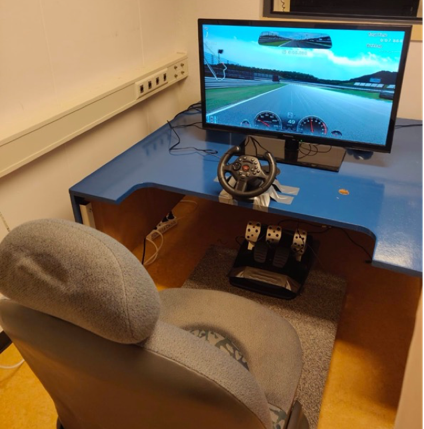
\includegraphics[width=\textwidth]{media/image1.png}
    \caption{The set-up of the driving simulator used in both the experimental driving and passive viewing control conditions. It consisted of a chair, steering wheel, pedals and a 23-inch flat screen. A PlayStation 3 and the game Gran Turismo \parencites{Yamauchi2013} were used to simulate the actual driving experience. Participants drove (or viewed a recorded video of) three laps on the Twin Motegi Course.}
    \label{fig:rId12}
  \end{fullwidth}
\end{figure}


\subsection{Procedure}



Before engaging in the experiment, participants were seated behind a desk with a laptop on which a short introductory text was displayed that informed them that the study was about multitasking while driving. After providing informed consent, participants next reported their driving experience. Following this, they were randomly assigned to the driving or control condition (see \emph{Driving simulation} for details), and asked to sit in the driver’s seat of the simulator where they were provided instructions for the driving simulation. Participants were then provided with a bowl of potato chips (10 grams, 50.8 kcal) and instructed to consume them all during the driving simulation. The chips used were Lays Classic salted potato chips. All participants consumed the entire 10 grams/50.8 kcal. Participants then completed the driving simulation. Following the driving simulation, participants returned to the desk to report their ratings, stress levels, age, sex, and ethnicity on the laptop. Participants were then instructed to wait in the room while the experimenter collected debriefing forms from the adjacent room (wait time held constant at three minutes), and that if they wanted, they could eat the rest of the potato chips (the remaining 15 g (76.2 kcal) from the 25 g party bag, in a bowl on the same desk). The Netherlands Nutrition Centre states 30 g as the average portion size of chips in the Netherlands \parencites{VoedingscentrumND}. Participants were told that these potato chips were left over from the party bag and that they were free to consume them all. Finally, all participants were debriefed, thanked, and compensated for their participation.



\subsection{Materials}



\subsubsection{Driving Simulation }



To create a realistic and demanding driving context, a set-up was built that consisted of a chair, steering wheel, pedals, and a 23-inch flat screen (see Fig.1). A PlayStation 3 and the game Gran Turismo \parencites{Yamauchi2013} were used to simulate a realistic driving experience. Participants were seated in the driving chair and it was explained how they could speed up, break and steer. Participants were asked to drive three laps on the Twin Ring Motegi course that consisted of two straight sections, a large bend and 2 sharp bends. Participants were told they should drive as well as they could. Driving the three laps took three minutes on average. If a participant took longer than 10 minutes to complete the laps the simulation was stopped, however, none of the participants took longer than 10 minutes to drive the three laps. To create a comparable situation in the control condition, the same driving simulator was used. The participants in the control group acted as co-driver/passenger and did not actually drive themselves. Instead, a three-minute recorded video was played, showing the exact same three laps of the Twin Ring Motegi course that the participants drove in the experimental driving condition.











\subsubsection{Driving Experience}



Three questions addressed participants’ driving experience: ‘How many years do you have your driver’s license?’, ‘How often do you drive on average per week?’ and ‘How many kilometers did you cover on average in the last year?’. The three items were answered on five-point Likert scales. These included respectively, driving years ranging from 1 (up to 1 year), increasing with each scale point with 1 year to a maximum of 5 (over 7 years); driving frequency ranging from 1 (once a week) increasing with each scale point with one time per week to a maximum of 5 (7 times per week); and driving distance ranging from 1 (1,000km per year) increasing with each scale point with 1,000km per year to a maximum of 5 (7,000 km per year).



\subsubsection{Taste Intensity}



Participants rated the potato chips on three items relating to taste intensity, namely ‘saltiness’, ‘sourness’, and ‘sweetness’, on seven-point Likert scales ranging from 1 (\emph{not at all}) to 7 (\emph{very}). Sweetness and sourness ratings were included as catch trials, to establish that participants were not merely guessing when assessing the potato chips’ flavor. Furthermore, the sweetness and sourness ratings serve as a baseline measure since we do not expect them to differ between conditions.



\subsubsection{Hedonic Rating }



Participants next rated the potato chips on three more items relating to hedonic experience, namely ‘quality’, ‘tastiness’, and ‘crunchiness’, on the same seven-point Likert scales ranging from 1 (\emph{not at all}) to 7 (\emph{very}).



\subsubsection{Stress levels}



Participants were asked five questions pertaining to their experiences of stress during the simulation: ‘How relaxed were you during the driving simulation?’ (reversed), ‘How much did you have the feeling that you were in control during the driving simulation?’ (reversed), ‘How rushed did you feel during the driving simulation?’, ‘How nervous were you during the driving simulation?’, and ‘How well did you perform during the driving simulation?’ (reversed). All questions were answered on a six-point Likert scale ranging from 1 (\emph{not at all}) to 6 (\emph{very}).



\subsubsection{Calories Consumed }



The number of calories consumed was determined by weighing the bowl with the remaining chips once the participant had left and subtracting this from its initial weight. The weight in gram was then multiplied by the amount of kcal/g (5.08).

\subsection{Data Preparation}



All data preparation steps and statistical analyses were performed in R \parencites{RCoreTeam2019} and can be retrieved from the OSF page: \href{https://osf.io/twg9r/}{osf.io/twg9r/}. Distribution of the variables was examined by visual inspection, Shapiro-Wilks test and Levene’s test. Since some of the variables were skewed, robust regression using the rlm function of the R package MASS was used throughout for consistency.



Robust regression was used to examine the differences between conditions unless otherwise specified (see Results). For each dependent variable (taste intensity, hedonic rating and number of calories consumed) we first estimated a full factorial model that included main effects and interaction of the experimental factor (Driving, Control) and Driving Experience. If the interaction term was not statistically significant, subsequently models with only the main effects of the experimental factor and Driving Experience were estimated. Afterwards, we calculated the Bayes Information Criterion (BIC) in order to see which model performed best.



Reliability analysis revealed saltiness was poorly associated with sourness and sweetness (Cronbach’s α = 0.31), as expected, and so these ratings were therefore examined separately. The items assessing hedonic rating and stress showed adequate reliability (Cronbach’s alphas of respectively .69 and .79) and were therefore averaged into two overall scores. The three items that assessed driving experience were only moderately associated (Cronbach’s α = 0.54), but driving distance correlated significantly with both frequency (\emph{r} = 0.48) and years of license (\emph{r} = 0.34), with the latter two being uncorrelated (\emph{r} = 0.06). Even though each item thus seemed to tap into a somewhat different aspect of driving experience, they were nevertheless averaged to form a broad index of driving experience.




Subsequent t-test analyses confirmed that driving experience in years, frequency and distance did not vary across conditions (\emph{t}s < 1.42, \emph{p}s > 0.153, so that these could be incorporated as moderator variables into the regression models for taste ratings and consumption. Table 1 depicts the raw means and standard deviations of the three Driving Experience items (years, frequency and distance) as a function of condition. Since driving experience was highly skewed towards the lower end (see Figure 3a in the Supplement section), quartile scores were used in the analyses.



Control analyses showed that men had more driving experience (\emph{M} = 2.10, \emph{SD} = 0.71) than women (\emph{M} = 1.71, \emph{SD} = 0.76; \emph{F}(1,114) = 6.30, \emph{p }= 0.01). Moreover, men consumed more calories than women irrespective of the experimental condition (men: \emph{M} = 100.0 kcal, \emph{SD} = 27.9; women: \emph{M} = 71.7 kcal, \emph{SD} = 25.0; \emph{b }= -9.09, \emph{SE }= 2.04, \emph{t}(111) = -4.45, \emph{p} > .001). Therefore, we corrected for gender in all our analyses.





\begin{table}[t]
  \begin{fullwidth}
    \caption{ Means and standard deviations of driving experience (in years, distance and frequency) as a function of condition (driving; control).}
    \label{tab:tab1}
    \begin{tabularx}{\linewidth}{@{} X X X X @{}}
      \toprule

      \textbf{Condition} & \textbf{Driving Years}\textsuperscript{\textbf{1}}
                         & \textbf{Driving }\newline\textbf{Distance}         & \textbf{Driving }\newline \textbf{Frequency}              \\
      \midrule

      Driving            & 2.13 (1.23)                                        & 1.90 (1.28)                                  & 1.45 (.81) \\

      Control            & 2.39 (1.17)                                        & 1.63 (1.02)                                  & 1.53 (.86) \\
      \bottomrule
    \end{tabularx}

    \textsuperscript{1} \emph{\small The driving experience items were answered on five-point Likert scales ranging from respectively 1 (up to 1 year/once a week /1000km per year) to 5 (over 7 years/ 7 times per week /7000 km per year).}

  \end{fullwidth}
\end{table}



\section{Results}



\subsection{Effects of Driving on Calories consumed }





Table 2 and Figure 2 depict the mean and standard deviation/error for potato chips consumed in kcal during the driving manipulation and the follow-up free consumption test as a function of condition (Driving; Control).


Inspection of the histograms revealed that the number of calories consumed was not normally distributed, but had a bimodal distribution with many observations at the scale extremes (50.8, 127.0; see supplemental Fig. S6.b for histograms per condition). More specifically, during the free consumption period 52\% of participants consumed no chips and 20\% of participants consumed all of the chips. Given how many participants consumed the maximum amount of chips available, it is likely that the mean consumption amount would have been higher if it had not been restricted (i.e., censoring effect is likely). Therefore, we applied Tobit regression analyses\footnote{ We also analyzed the number of calories consumed using robust regression models. These yielded comparable results, see: \url{osf.io/twg9r/.}} \parencites[i.e., censored regression models][]{Tobin1958}, using the R package censReg \parencites{Henningsen2010}.



This Tobit regression analysis with calories consumed as dependent variable and main effects and interaction of the experimental factor (Driving, Control) and Driving Experience showed no significant interaction term, so a model with only main effects was estimated. There was a significant main effect of the driving manipulation, \emph{b = }-19.43, \emph{p = }0.026. As hypothesized, participants consumed more potato chips when driving (\emph{M }= 84.3 kcal, \emph{SE }= 4.11), compared to passively watching the same route (\emph{M }= 72.9 kcal, \emph{SE }= 3.24). Driving Experience did not have a main effect. The BIC for the model with only main effects was lower than the model with the interaction term (BIC 3.15).




\subsection{Effects of Driving on Taste Intensity }



Table 2 and Figure 2 depict the means and standard deviations for all taste intensity ratings as a function of condition (Driving; Control).








Robust regression analyses incorporating main effects and interaction of the experimental factor (Driving, Control) and Driving Experience were conducted to examine the effects on saltiness ratings. The BIC for the model with only main effects was lower than the model with the interaction term (BIC 2.67). Contrary to our first hypothesis, we did not observe a significant main effect of condition, \emph{b }= 0.42, \emph{SE }= .23, \emph{t}(111) = 1.84, \emph{p }= 0.067. As predicted, participants rated the potato chips as less salty when they were driving themselves (\emph{M }= 4.43, \emph{SE }= 0.16), than when they were attending a recording of the same route being driven by someone else (\emph{M }= 4.74, \emph{SE }= 0.15), but this difference did not reach the threshold for significance. Control analyses confirmed that the driving manipulation likewise did not significantly impact participants’ sourness and sweetness ratings (\emph{t}s < 0.3, \emph{p}s > .54) with very similar intensity ratings across conditions (see Fig.2). The potato chips were generally perceived to be minimally sweet (\emph{M = }2.01, \emph{SD = }1.15) and sour (\emph{M = }1.72, \emph{SD = }0.96). Taken together, even though the intensity ratings showed the expected pattern, we found no robust proof that driving interfered with participants’ processing of the saltiness of the chips.



There was no main effect or interaction effect of Driving Experience.





\begin{table*}
  \begin{fullwidth}
    \caption{Means and standard deviations of the various taste ratings (1 - not at all to 7 - very) and amount consumed in kcal as a function of condition (driving; control).}
    \label{tab:tab2}


    \begin{tabularx}{\textwidth}{@{} l l >{\RaggedRight\arraybackslash}X l l l l >{\RaggedRight\arraybackslash}X @{}}
      \toprule
      \textbf{Condition} & \textbf{Salty} & \textbf{Sweet}
                         & \textbf{Sour}  & \textbf{Quality}                  & \textbf{Tasty} & \textbf{Crunchy} &
      \textbf{Total Calories Consumed}                                                                              \\

      \midrule

      Driving            & 4.43 (1.19)    & 2.00 (1.27)  \newline 1.79 (1.04) & 1.79 (1.04)
                         & 4.85 (1.14)    & 5.17 (1.35)                       & 5.12 (1.20)    & 84.3 (31.1)        \\

      Control            & 4.74 (1.15)    & 2.05 (1.03)                       & 1.69 (0.90)    &
      4.67 (1.37)        & 4.98 (1.40)    & 5.22 (1.13)                       & 72.9 (24.7)                         \\
      \bottomrule
    \end{tabularx}
  \end{fullwidth}
\end{table*}


\begin{figure}[t!]
  \begin{fullwidth}
    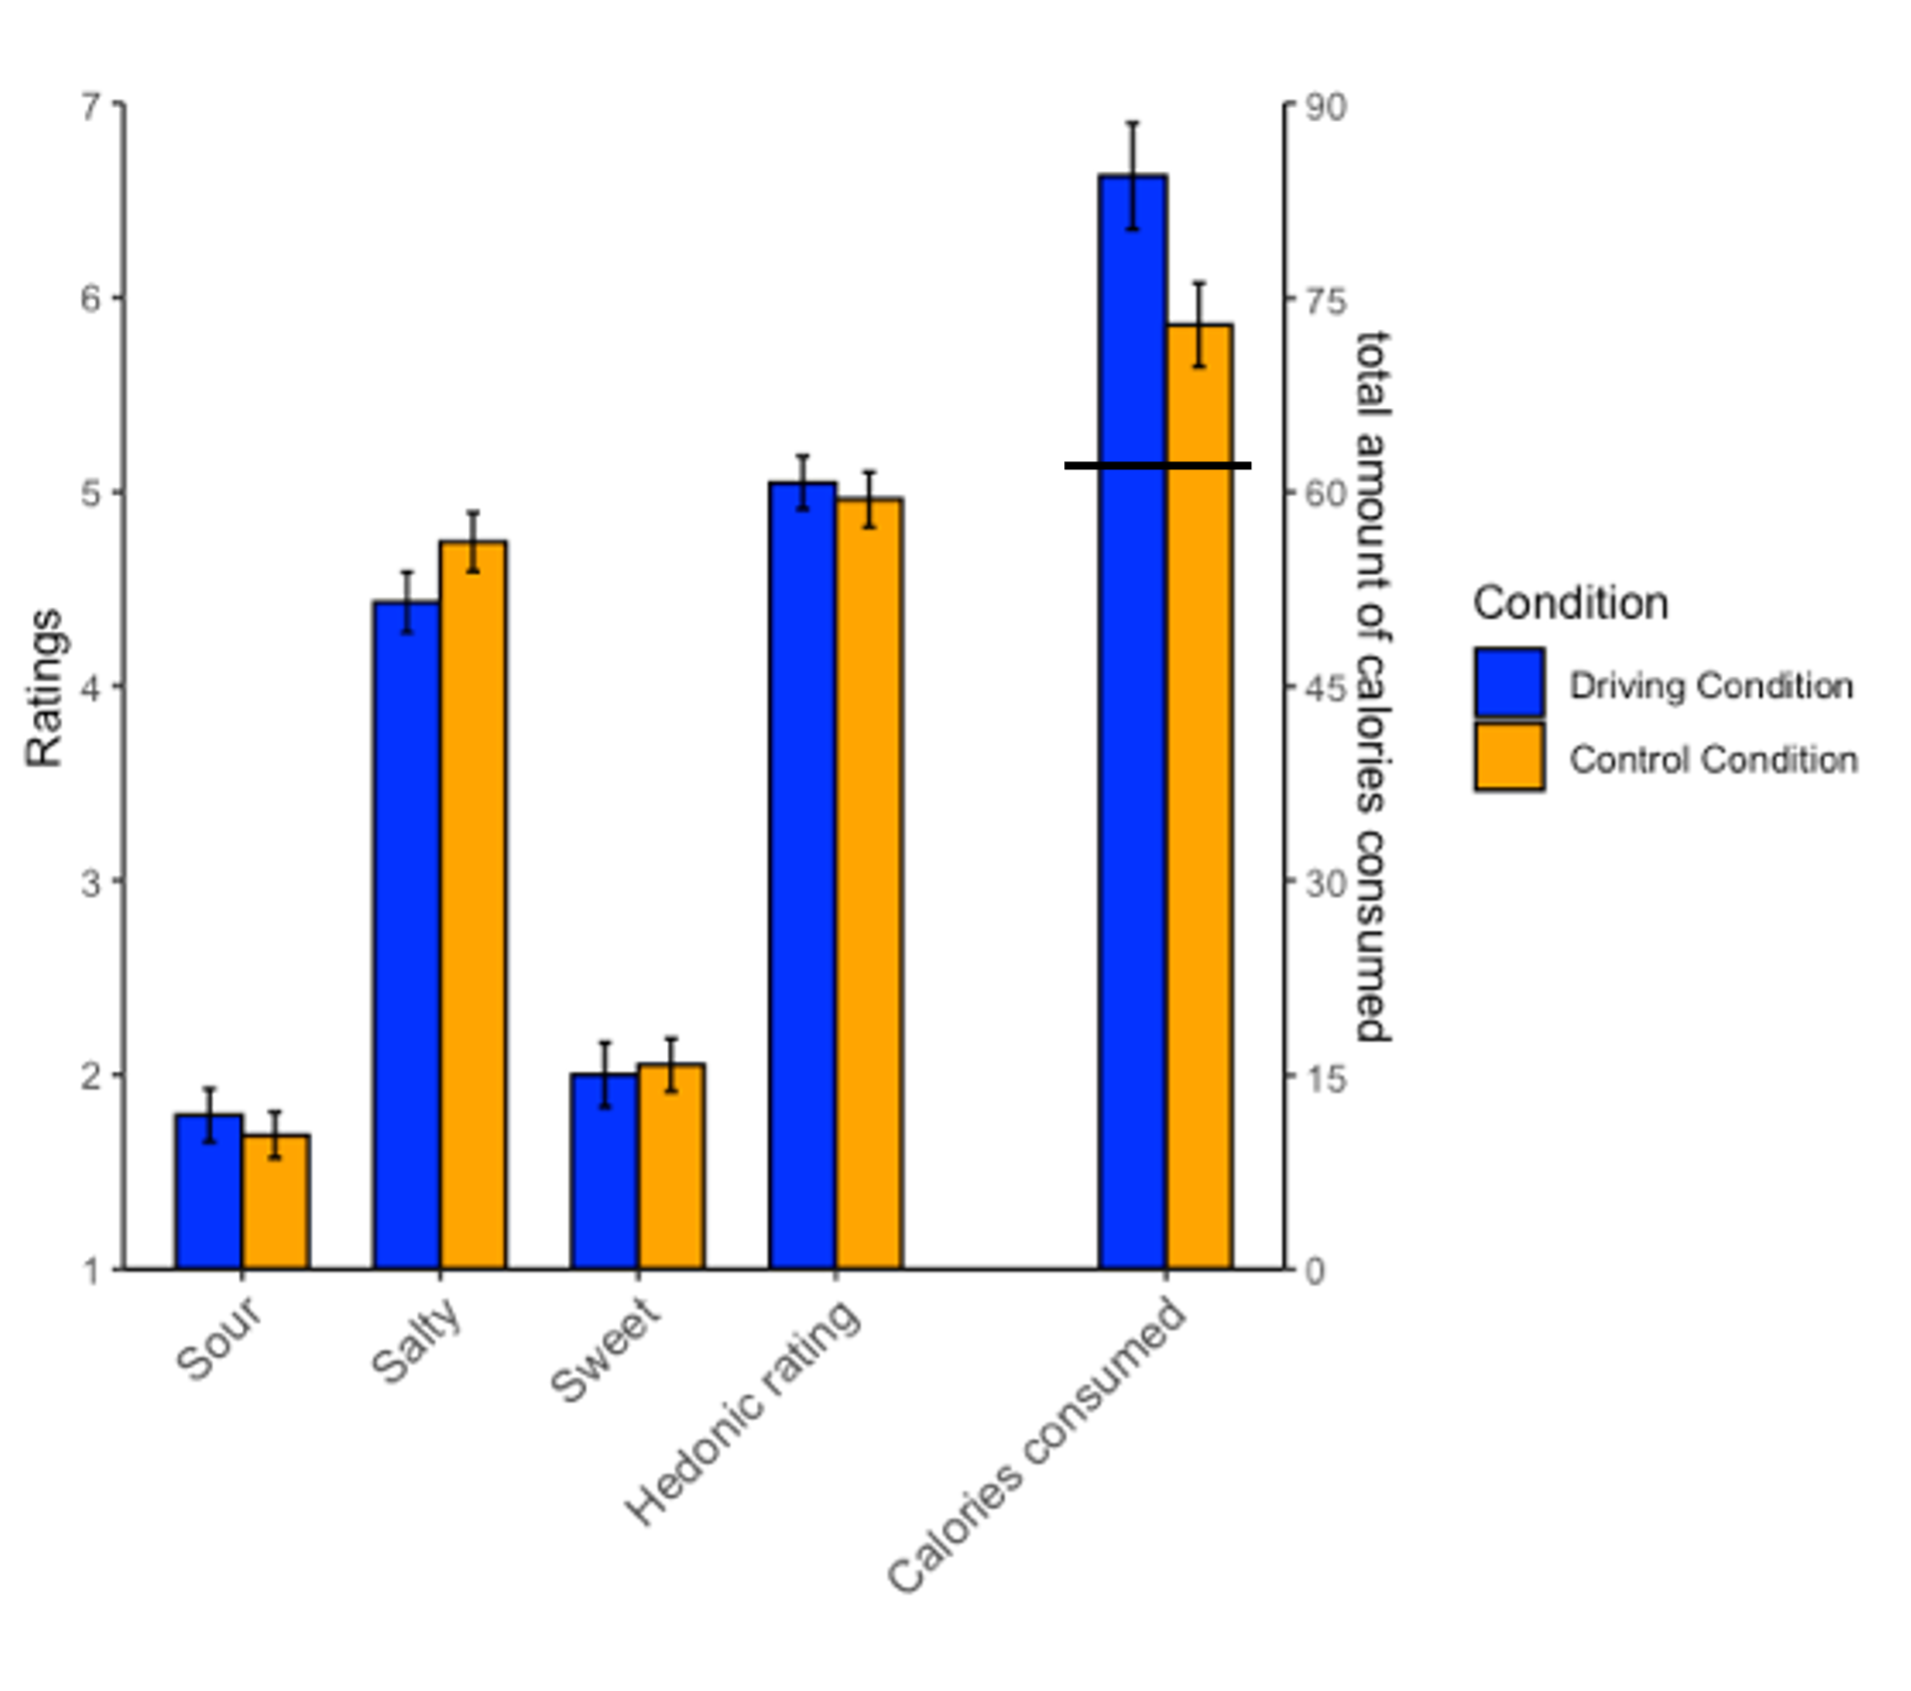
\includegraphics[width=\linewidth]{media/image2.png}
    \caption{Mean of taste intensity ratings, hedonic ratings and total calories of chips consumed per condition. “Hedonic rating” here reflects the mean of the “quality”, “crunchy” and “tasty” ratings. Total amount of calories includes the standard amount of 50.8 kcal of chips eaten during the manipulation, as indicated by the horizontal black line. Error bars reflect standard error.}
  \end{fullwidth}
  \label{fig:rId14}

\end{figure}









\subsection{Explorations of Hedonic Rating and Driving-induced Stress as Alternative Explanation }

\vspace*{-1\baselineskip}

We also explored whether driving altered hedonic aspects of the consumption experience. A robust regression model with hedonic rating as dependent variable and main effects and interaction of the experimental factor (Driving, Control) and Driving Experience was estimated. Table 2 depicts the means and standard deviations for the three hedonic ratings as a function of condition (Driving; Control). These showed that participants rated hedonic aspects no different in the driving condition (\emph{M} = 5.08, \emph{SE} = 0.41) than the control condition (\emph{M }= 4.95, \emph{SE }= 0.42, \emph{b }= -0.18, \emph{p }= 0.782). When the items were analyzed separately, this did not yield any significant differences either (\emph{p}s>0.356). Finally, driving experience did not significantly impact hedonic rating (\emph{p}=0.344) nor was there a significant interaction between Driving Experience and condition on hedonic rating (\emph{p }= 0.125).



We next examined whether the effects of driving on perception and consumption resulted from driving-induced stress as opposed to distraction. Table 3 depicts the means and standard deviations for the five stress ratings as a function of condition (Driving; Control). These revealed that all five items were affected by the driving manipulation; participants were significantly less relaxed, and felt significantly more in control, rushed, nervous, and performing well while driving than while in the passive viewing condition, \emph{t}s>2.93, \emph{p}s<0.020. This confirms that driving compared to passive viewing heightened participants’ stress levels. There was no interaction between Driving Experience and the driving manipulation on perceived stress levels (\emph{p }= 0.17).

\begin{table*}[t]
  \begin{fullwidth}
    \caption{Means and standard deviations (between brackets) of the various stress ratings (1- not at all to 7 – very) as a function of condition (driving; control).}
    \label{tab:tab3}
    \begin{tabularx}{\textwidth}{@{} X X X X X X  @{}}
      \toprule
      \textbf{Condition} & \textbf{Relaxed}
                         & \textbf{In control} & \textbf{Rushed}
                         & \textbf{Nervous}    & \textbf{Performed well}

      \\
      \midrule

      Driving            & 3.28 (1.32)         & 3.20 (1.30)             & 3.82 (1.24) & 3.17 (1.45)
                         & 3.95 (.95)                                                                \\

      Control            & 4.44 (1.34)         & 1.56 (.88)              & 2.88 (1.35) & 2.56 (1.41)
                         & 2.63 (1.07)                                                               \\
      \bottomrule
    \end{tabularx}
  \end{fullwidth}
\end{table*}







To test whether the effect of condition on the amount of food consumed could be explained by the difference in experienced stress, a Tobit regression analysis was performed with calories consumed as the dependent variable and the main effects and interactions of the experimental factor (Driving, Control), stress, and Driving Experience. Since the full factorial did not show a significant effect of the interaction term with Driving Experience, subsequently a model was estimated with calories consumed as the dependent variable and the main effects and interactions of the experimental factor (Driving, Control) and stress and only a main effect for Driving Experience (BIC 9.43). The analysis showed a main effect for both conditions, \emph{b }= -25.82, \emph{SE }= 32.14, \emph{t }=-2.60, \emph{p }= 0.009, and stress, \emph{b }= -15.83, \emph{SE }= 7.60, \emph{t }= -2.08, \emph{p }= 0.037. Interestingly, the effect of stress on consumption was negative, which means that participants who felt more stressed ate less. This suggests that increases in stress did not explain increased consumption following driving. Additionally, there was a significant interaction effect of driving manipulation and stress on calories consumed: \emph{b }= 18.22, \emph{SE }= 9.29, \emph{t }= 1.96, \emph{p }= 0.038. Although there was no significant main effect of stress on consumption when the analyses were done in the respective conditions, a Fischer r to z comparison confirmed that the slopes of the effect of stress on calories consumed in the driving and control condition were different, \emph{Z} = 2.00, \emph{p} = 0.05. In the driving condition stress had a stronger negative effect on calories consumed (\emph{r} = -0.37) compared to the control condition (\emph{r }= -0.12). There was no significant main effect of stress on consumption when the analyses were done in the respective conditions. When added as covariate to the overall regression model, stress did not explain the main effect of driving on calories consumed.



In conclusion, stress had a negative effect on consumption. So, even though participants felt more stressed in the driving condition, stress did not account for the difference in calories consumed between the driving and control condition.



There was no effect of stress on saltiness ratings or any interactions between stress and condition or driving experience on saltiness ratings (all \emph{p}s >0.35). However, when stress was entered into the model, the effect of condition on saltiness ratings became significant (\emph{b }= 0.54, \emph{SE = }0.26, \emph{t}(111) = 2.035\emph{, p }= 0.0454).\footnote{ Restrained Eating as measured by the Restrained Eating Scale \parencites{Polivy1978} was examined as a potential moderator as well. There was no difference in Restrained Eating between the driving (M=13.0; SD=5.82) and control condition (\emph{M} = 11.9; \emph{SD} = 4.76). Restrained Eating did not interact with any of the variables of interest. Adding total Restrained Eating score as a covariate did not change the overall pattern of results, see: \href{https://osf.io/twg9r/}{osf.io/twg9r/}.}



In order to examine the relationships between all factors of interest and to take into account that driving experience and stress are assessed by multiple items, we used structural equation modeling (SEM) to estimate path models using the lavaan package in R \parencites{Rosseel2012}. Figure 6 in the supplementary section depicts the model that was tested. Calories consumed was the dependent variable, driving condition was included as a predictor and taste perception (saltiness ratings) and stress were assessed as possible mediators between driving condition and calories consumed. Stress and driving experience were modeled as latent variables. Furthermore, gender was added to the model as a control variable. Since lavaan does not support interactions with latent variables, no interactions were modeled. Model fit indices show a poor fit for the model (\emph{CFI} = 0.69; \emph{SRMR} = 0.12; \emph{RMSEA} = 0.14 (90\% CI: 0.12 to 0.17). The model showed a significant effect of driving condition on calories consumed (\emph{b }= 13.62, \emph{SE = }6.14, \emph{p }= 0.027) but did not indicate stress or saltiness ratings as a mediator of this effect via a direct or indirect path (Figure 6; analysis script on \href{https://osf.io/twg9r/}{OSF}).



\section{General Discussion}




In this study we aimed to build on previous studies that found that distraction increased consumption by examining possible explanations of the effect in a practically relevant setting. To do so, in a simulated driving experiment, we examined whether snacking while driving would result in greater consumption afterwards. We furthermore investigated whether this effect could be explained by reduced taste intensity while driving or by driving-induced stress.



In support of our predictions, participants who engaged in the driving simulation while consuming potato chips, consumed more potato chips during a follow-up free consumption test than participants who merely watched a recording. There were some indications that the driving simulation lowered the saltiness ratings of the chips. Other sensory ratings and hedonic ratings were unaffected by driving.



Many different (complementary) explanations have been proposed for the mechanism which makes people consume more after or during distracted consumption, including reduced memory for food intake or health goals, disrupted influence of satiation, and dishabituation \parencites{Forde2018}{Robinson2013}. In the current study, we found some indications that lowered taste perception may be an interesting component to consider when studying the mechanism behind overconsumption after distracted eating.

\begin{originalPurpose}
  In this study, we aimed to examine the effect of eating while driving, and potential underlying mechanisms. We hypothesized that eating while driving would reduce taste perception, which would in turn cause participants to overconsume afterwards to compensate. Based on previous research, we expected that taste perception, but not hedonic preference, would be diminished during distracted consumption. We furthermore wanted to examine the effect of stress experienced during the driving simulation as an alternative explanation.
\end{originalPurpose}


Our finding that distraction may reduce perceptions of saltiness supports previous literature demonstrating this effect \parencites{Wal2013}{Liang2018}{Duif2020}. As taste intensity has been found to correlate negatively with food intake \parencites{Forde2013}, lowered experienced taste intensity during distracted eating may lead to increased food consumption. Furthermore, when distracted, taste information may not be processed in a way that leads to satisfaction or satiation. For example, consuming a high calorie drink under high perceptual load led to lower satiety than when the same drink was consumed under low perceptual load \parencites{Morris2020}. Future studies could examine the effect of distracted consumption on satiation/satiety and how this relates to taste perception and other outcomes.



Perceived stress was examined as an alternative explanation of the effect of distracted consumption on subsequent consumption. Whereas participants reported more stress after driving than after watching someone else drive, self-reported stress yielded an opposite effect on consumption, with participants consuming \emph{fewer} rather than more potato chips. The phenomenon that acute stress can reduce food intake has been attributed to physiologic changes that occur after acute stress and that might be expected to temporarily reduce food intake, e.g., slowed gastric emptying and shifting of blood from the gastrointestinal tract to muscles \parencites{Torres2007}.


Several previous studies have found an effect of restrained eating on the relationship between stress and consumption \parencites{Wallis2004}{Wallis2009}. However, we did not find an effect of restrained eating on consumption or any interaction between restrained eating, stress or driving manipulation. This could possibly be explained by the fact that restrained eating scores in our sample were low.



In conclusion, higher perceived stress was associated with lower consumption of potato chips. Therefore, the finding that the driving manipulation increased intake could be not accounted for by the driving induced stress.



A strength of the current study is the use of a realistic and practically relevant distractor and consumption situation. This study aimed for a control condition that matched the sensory input during driving and thus only differed from the experimental condition in the mental load and stress induced. As a result, the participants in the control condition were probably still somewhat distracted and this might have created a conservative test of our hypotheses. However, this way, any differences in consumption and perceived taste intensity between the conditions could be attributed to differences in the availability of mental capacity. It is possible that the smaller effect sizes have caused our study to be underpowered to detect the effect of driving condition on saltiness ratings. Future research could examine variations in mental load and stress further by comparing different levels of distraction during consumption, e.g., high distraction, low distraction, no distraction and targeted attention through mindful eating instructions in a larger sample.



The current study also has its limitations. Whereas standardization of the consumption amount during the driving manipulation allowed us to examine differences in compensatory consumption, one limitation of the study is the limited amount that could be consumed later. The mean difference in the amount of potato chips consumed after driving or passively watching was only 11 kcal. However, these 11 kcal were consumed in addition to the 50.8 kcal that participants already ate during the driving distraction or passively viewing. In addition, a substantial proportion of the sample consumed the entire additional 15 grams or 76 kcal, which might indicate that they would have consumed more had they had the opportunity to do so. To further examine the magnitude and practical relevance of the compensatory consumption effect, future studies could examine ad libitum intake following distracted eating.



Although participants were requested not to eat in the two hours prior to the start of the study, subjective hunger was not assessed. However, since participants were randomly assigned to the driving or control condition, possible variability in hunger status is unlikely to have caused the difference in subsequent consumption between conditions.



We did not assess how much experience with playing video games participants had. In addition to driving experience, this may have affected how challenging the driving simulation was for participants.



Lastly, the relatively young age, low driving experience, high education level and unbalanced gender ratio of our sample limits the generalizability of our results. Furthermore, ethnicity was not assessed. Future studies could extend our findings in broader samples that are more representative of the general population.

\section{Conclusion}



Using a realistic but lab-controlled driving simulation, the findings reported here provide additional support for the notion that distracting consumption settings may have long-term health implications, through their contribution to overconsumption of unhealthy products. This pushes the need for a better understanding of what these settings look like in people’s daily lives and how consumption settings can be changed. The current research provides some preliminary evidence that taste perception, and especially perceived taste intensity, may be a relevant aspect to consider when examining the mechanism through which distracted eating leads to overconsumption.

\section{Funding}
This research was supported by an Open Research Area grant (Dutch Research Council Grant No. 464-18-105; German Research Foundation Grant HO 4175/7-1).


\section{Author contributions}



LFvD developed the study design and oversaw the data collection; FvM and LFvD performed the primary data analyses and HvS provided additional analyses; FvM, LFvD, HvS, SLM, and WH prepared the manuscript; all authors provided critical revisions and approved the final version of the manuscript.


\section{Acknowledgements}



We thank Maureen Botz, Lukas Sutorius and Marit van Wijncoop for their assistance during data collection.


\printbibliography



% Antoun, M., Edwards, K. M., Sweeting J., & Ding, D. (2017). The acute physiological stress response to driving: A systematic review. \emph{PLoS ONE 12}(10), Article e0185517\emph{.} https://doi.org/10.1371/journal.pone.0185517



% Arch, J. J., Brown, K. W., Goodman, R. J., Della Porta, M. D., Kiken, L. G., & Tillman, S. (2016). Enjoying food without caloric cost: The impact of brief mindfulness on laboratory eating outcomes. \emph{Behaviour Research and Therapy}, \emph{79}, 23-34.



% Blass, E. M., Anderson, D. R., Kirkorian, H. L., Pempek, T. A., Price, I., & Koleini, M. F. (2006). On the road to obesity: Television viewing increases intake of high-density foods. \emph{Physiology & Behavior, 88}(4-5), 597-604.



% Bolhuis, D. P., Lakemond, C. M., de Wijk, R. A., Luning, P. A., & de Graaf, C. (2012). Effect of salt intensity in soup on ad libitum intake and on subsequent food choice. \emph{Appetite, 58}(1), 48-55.



% Crespo, C. J., Smit, E., Troiano, R. P., Bartlett, S. J., Macera, C. A., & Andersen, R. E. (2001). Television watching, energy intake, and obesity in US children: results from the third National Health and Nutrition Examination Survey, 1988-1994. \emph{Archives of Pediatrics & Adolescent Medicine}, \emph{155}(3), 360-365.



% DiFeliceantonio, A. G., Coppin, G., Rigoux, L., Thanarajah, S. E., Dagher, A., Tittgemeyer, M., & Small, D. M. (2018). Supra-additive effects of combining fat and carbohydrate on food reward. \emph{Cell Metabolism}, \emph{28}(1), 33-44.



% Dingus, T. A., Guo, F., Lee, S., Antin, J. F., Perez, M., Buchanan-King, M., & Hankey, J. (2016). Driver crash risk factors and prevalence evaluation using naturalistic driving data. \emph{Proceedings of the National Academy of Sciences}, \emph{113}(10), 2636-2641.



% Dubois, L., Farmer, A., Girard, M., & Peterson, K. (2008). Social factors and television use during meals and snacks is associated with higher BMI among pre-school children. \emph{Public Health Nutrition}, \emph{11}(12), 1267-1279.



% Duif, I., Wegman, J., Mars, M. M., de Graaf, C., Smeets, P. A., & Aarts, E. (2020). Effects of distraction on taste-related neural processing: A cross-sectional fMRI study. \emph{The American Journal of Clinical Nutrition}, \emph{111}(5), 950-961.



% FoodShopper Monitor (2018). \emph{FSIN FoodShopper Monitor 2019}. FoodService Instituut Nederland. \emph{https://fsin.nl/foodshoppermonitor }



% Forde, C. G. (2018). From perception to ingestion: The role of sensory properties in energy selection, eating behaviour and food intake. \emph{Food Quality and Preference}, \emph{66}, 171-177.



% Forde, C. G., van Kuijk, N., Thaler, T., de Graaf, C., & Martin, N. (2013). Oral processing characteristics of solid savoury meal components, and relationship with food composition, sensory attributes and expected satiation. \emph{Appetite, 60,} 208–219.



% Henningsen, A. (2010). Estimating censored regression models in R using the censReg Package. \emph{R Package Vignettes, 5}, 1-12.



% Hoffmann-Hensel, S. M., Sijben, R., Rodriguez-Raecke, R., & Freiherr, J. (2017). Cognitive load alters neuronal processing of food odors. \emph{Chemical Senses}, \emph{42}(9), 723-736.



% Higgs, S., & Donohoe, J.E. (2011). Focusing on food during lunch enhances lunch memory and decreases later snack intake. \emph{Appetite, 57, }202–6.



% Higgs, S., Williamson, A.C., & Attwood, A.S. (2008). Recall of recent lunch and its effect on subsequent snack intake. \emph{Physiology & Behavior}, \emph{94, }454–62.



% Higgs, S., & Woodward, M. (2009). Television watching during lunch increases afternoon snack intake of young women. \emph{Appetite}, \emph{52}, 39-43.



% Hirschberg, C., Rajko, A., Schumacher, T., & Wrulich, M. (2016, November 9). The changing market for food delivery. Mckinsey and Co. https://www.mckinsey.com/industries/technology-media-and-telecommunications/our-insights/the-changing-market-for-food-delivery



% Irwin, C., Monement, S., & Desbrow, B. (2015). The influence of drinking, texting, and eating on simulated driving performance. \emph{Traffic Injury Prevention}, \emph{16}, 116-123.



% Liang, P., Jiang, J., Ding, Q., Tang, X., & Roy, S. (2018). Memory load influences taste sensitivities. \emph{Frontiers in Psychology, 9}, Article 2533.



% McCrickerd, K., & Forde, C. G. (2016). Sensory influences on food intake control: moving beyond palatability. \emph{Obesity Reviews}, \emph{17}(1), 18-29.



% Morris, J., Vi, C. T., Obrist, M., Forster, S., & Yeomans, M. R. (2020). Ingested but not perceived: Response to satiety cues disrupted by perceptual load. \emph{Appetite}, \emph{155}, Article 104813.



% Moskowitz, H. R. (1972). Perceptual changes in taste mixtures. \emph{Perception & Psychophysics, 11(4), }257-262.



% Ogden, J., Oikonomou, E., & Alemany, G. (2013). Distraction, restrained eating and disinhibition: An experimental study of food intake and the impact of ‘eating on the go’. \emph{Journal of Health Psychology}, \emph{22}, 39-50.



% Oldham-Cooper, R. E., Hardman, C. A., Nicoll, C. E., Rogers, P. J., & Brunstrom, J. M. (2010). Playing a computer game during lunch affects fullness, memory for lunch, and later snack intake. \emph{The American Journal of Clinical Nutrition}, \emph{93}, 308-313.



% Polivy, J., Herman, C. P., & Warsh, S. (1978). Internal and external components of emotionality in restrained and unrestrained eaters. \emph{Journal of Abnormal Psychology}, \emph{87(5)}, 497-504.



% R Core Team (2019). \emph{R: A language and environment for statistical computing}. R Foundation for Statistical Computing. \href{https://www.R-project.org/}{https://www.R-project.org/}.



% Reichenberger, J., Kuppens, P., Liedlgruber, M., Wilhelm, F. H., Tiefengrabner, M., Ginzinger, S., & Blechert, J. (2018). No haste, more taste: An EMA study of the effects of stress, negative and positive emotions on eating behavior. \emph{Biological Psychology}, \emph{131}, 54-62.



% Robinson, E., Aveyard, P., Daley, A., Jolly, K., Lewis, A., Lycett, D., & Higgs, S. (2013). Eating attentively: A systematic review and meta-analysis of the effect of food intake memory and awareness on eating. \emph{The American Journal of Clinical Nutrition, 97}, 728-742.



% Robinson, E., Kersbergen, I., & Higgs, S. (2014). Eating “attentively” reduces later energy consumption in overweight and obese females. \emph{British Journal of Nutrition, 112}, 657–61.



% Rolls, E. T., & Grabenhorst, F. (2008). The orbitofrontal cortex and beyond: From affect to decision-making. \emph{Progress in Neurobiology}, \emph{86}(3), 216-244.



% Rosseel, Y. (2012). Lavaan: An r package for structural equation modeling and more. Version 0.5–12 (BETA). \emph{Journal of Statistical Software, 48}(2), 1–36. https://doi.org/10.18637/jss.v048.i02



% Rousseeuw, P. J., Croux, C., Todorov, V., Ruckstuhl, A., Salibian-Barrera, M., Sobal, J., Bisogni, C. A., Devine, C. M., & Jastran, M. (2006). A conceptual model of the food choice process over the life course. \emph{Frontiers in Nutritional Science}, \emph{3}, 1-18.



% Small, D. M., & DiFeliceantonio, A. G. (2019). Processed foods and food reward. \emph{Science}, \emph{363}(6425), 346-347.



% Spence, C., & Shankar, M. U. (2010). The influence of auditory cues on the perception of, and responses to, food and drink. \emph{Journal of Sensory Studies}, \emph{25}(3), 406-430.



% Stafford, L. D., & Dodd, H. (2013). Music increases alcohol consumption rate in young females. \emph{Experimental and Clinical Psychopharmacology}, \emph{21}(5), 408-415.



% Stroebele, N., & de Castro, J. M. (2006). Listening to music while eating is related to increases in people's food intake and meal duration. \emph{Appetite}, \emph{47}, 285-289.



% Stutts, J., Feaganes, J., Reinfurt, D., Rodgman, E., Hamlett, C., Gish, K., & Staplin, L. (2005). Driver's exposure to distractions in their natural driving environment. \emph{Accident Analysis & Prevention}, \emph{37}(6), 1093-1101.



% Tang, D. W., Fellows, L. K., & Dagher, A. (2014). Behavioral and neural valuation of



% foods is driven by implicit knowledge of caloric content. \emph{Psychological Science}, \emph{25}(12), 2168-2176.



% Torres, S. J., & Nowson, C. A. (2007). Relationship between stress, eating behavior, and obesity. \emph{Nutrition}, \emph{23}(11-12), 887-894.



% van der Wal, R. C., & van Dillen, L. F. (2013). Leaving a flat taste in your mouth: Task load reduces taste perception. \emph{Psychological Science}, \emph{24}, 1277-1284.



% Voedingscentrum. (n.d.) \emph{Wat is de voedingswaarde van chips op basis van aardappelmeel}. https://www.voedingscentrum.nl/nl/service/vraag-en-antwoord/gezonde-voeding-en-voedingsstoffen/hoeveel-voedingswaarden-zitten-erin/chips-op-basis-van-aardappelmeel.aspx



% Wallis, D. J., & Hetherington, M. M. (2009). Emotions and eating. Self-reported and experimentally induced changes in food intake under stress. \emph{Appetite, 52(2)}, 355-362.



% Wallis, D. J., & Hetherington, M. M. (2004). Stress and eating: The effects of ego-threat and cognitive demand on food intake in restrained and emotional eaters. \emph{Appetite}, \emph{43}(1), 39-46.



% Yamauchi, K. (2013). \emph{Gran Turismo} [video game]. Sony Interactive Entertainment.



% Young, M. S., Mahfoud, J. M., Walker, G. H., Jenkins, D. P., & Stanton, N. A. (2008). Crash dieting: The effects of eating and drinking on driving performance. \emph{Accident Analysis & Prevention}, \emph{40}, 142-148.



% Zontone, P., Affanni, A., Bernardini, R., Del Linz, L., Piras, A., & Rinaldo, R. (2020). Stress evaluation in simulated autonomous and manual driving through the analysis of skin potential response and electrocardiogram signals. \emph{Sensors, 20(9)}, Article 2494.







\clearpage
\onecolumn

\section{Supplementary Tables and Figures}




\begin{table}[h]
  \caption{Means and standard deviations or \emph{N} of gender, age and nationality as a function of condition (driving; control).}
  \label{tab:s1}
  \begin{tabularx}{\textwidth}{@{} l l l X  @{}}

    \toprule
    \textbf{Condition*} &
    \textbf{Gender}     & \textbf{Age} &

    \textbf{Nationality }                                                                       \\
    \midrule

    Driving             & 15 M, 43 F   & 22.00 (2.66) & 29 Dutch, 8 German, 3 English, 18 other
    \\
    Control             & 15 M, 43 F   & 21.60 (3.02) & 39 Dutch, 8 German, 11 other
    \\
    \bottomrule
  \end{tabularx}
  \emph{\small  *There were no statistically significant differences between the groups.}
\end{table}






\begin{figure}[h!]

  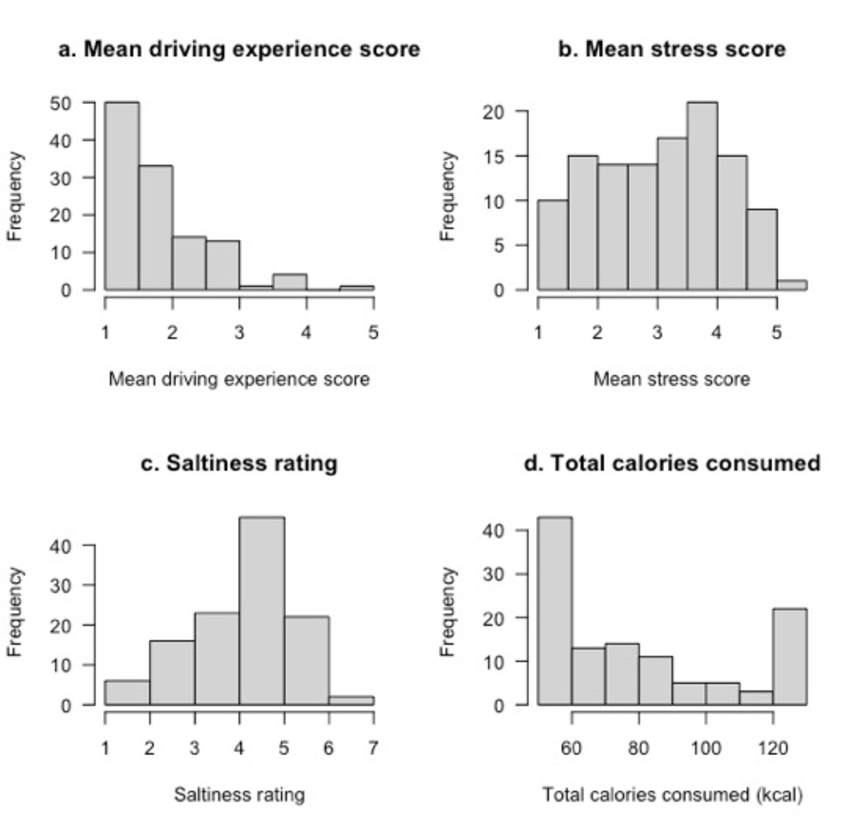
\includegraphics[width=.8\textwidth]{media/image3.pdf}
  \centering
  \caption{Histograms showing the distributions for a. mean Driving Experience, b. mean stress score, c. salt intensity rating, d. total amount of calories consumed.}

  \label{fig:rId25}
\end{figure}

\begin{figure}
  \centering
  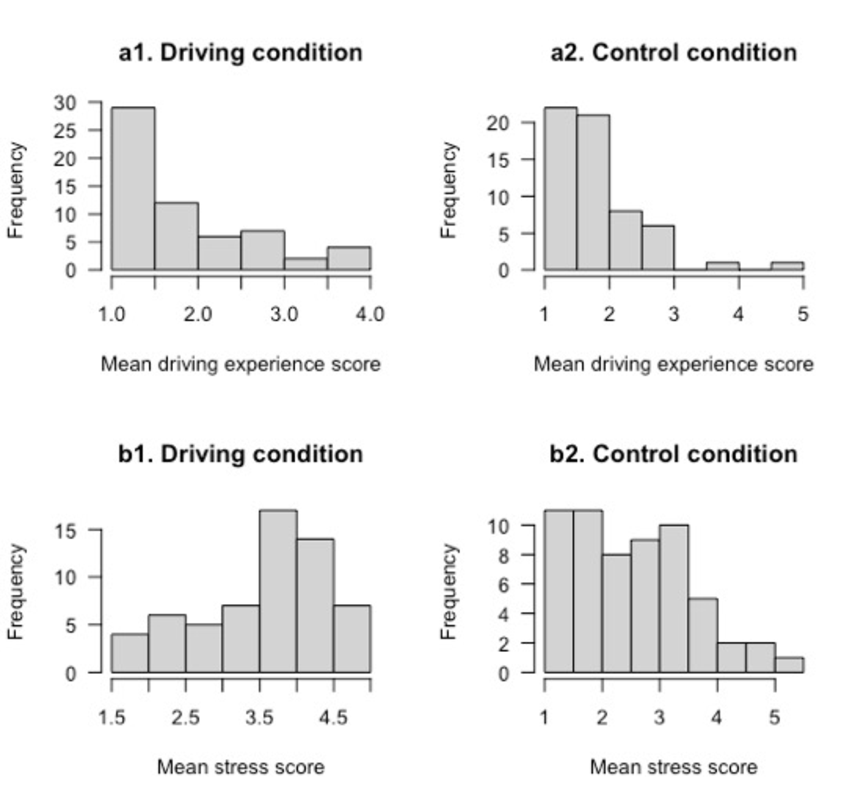
\includegraphics[width=.7\textwidth]{media/image4.pdf}
  \caption{Histograms showing the distributions per condition (Driving and Control) for a. mean Driving Experience, b. mean stress score.}

  \label{fig:rId26}

\end{figure}




\begin{figure}
  \centering
  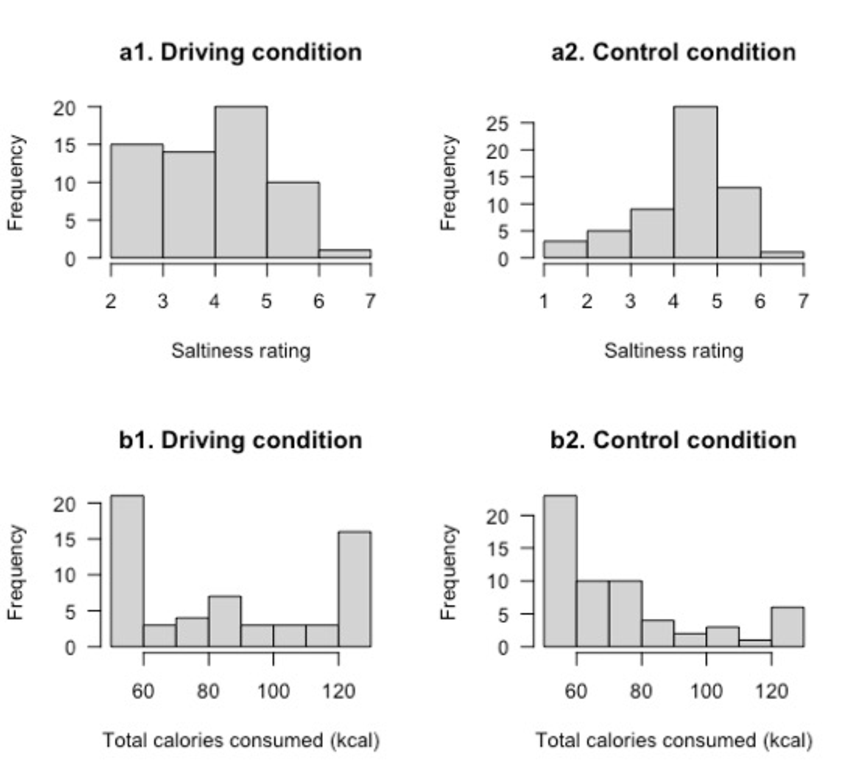
\includegraphics[width=.7\textwidth]{media/image5.pdf}
  \caption{Histograms showing the distributions per condition (Driving and Control) for a. salt intensity rating, b. total amount of calories consumed.}

  \label{fig:rId27}

\end{figure}


\begin{figure}

  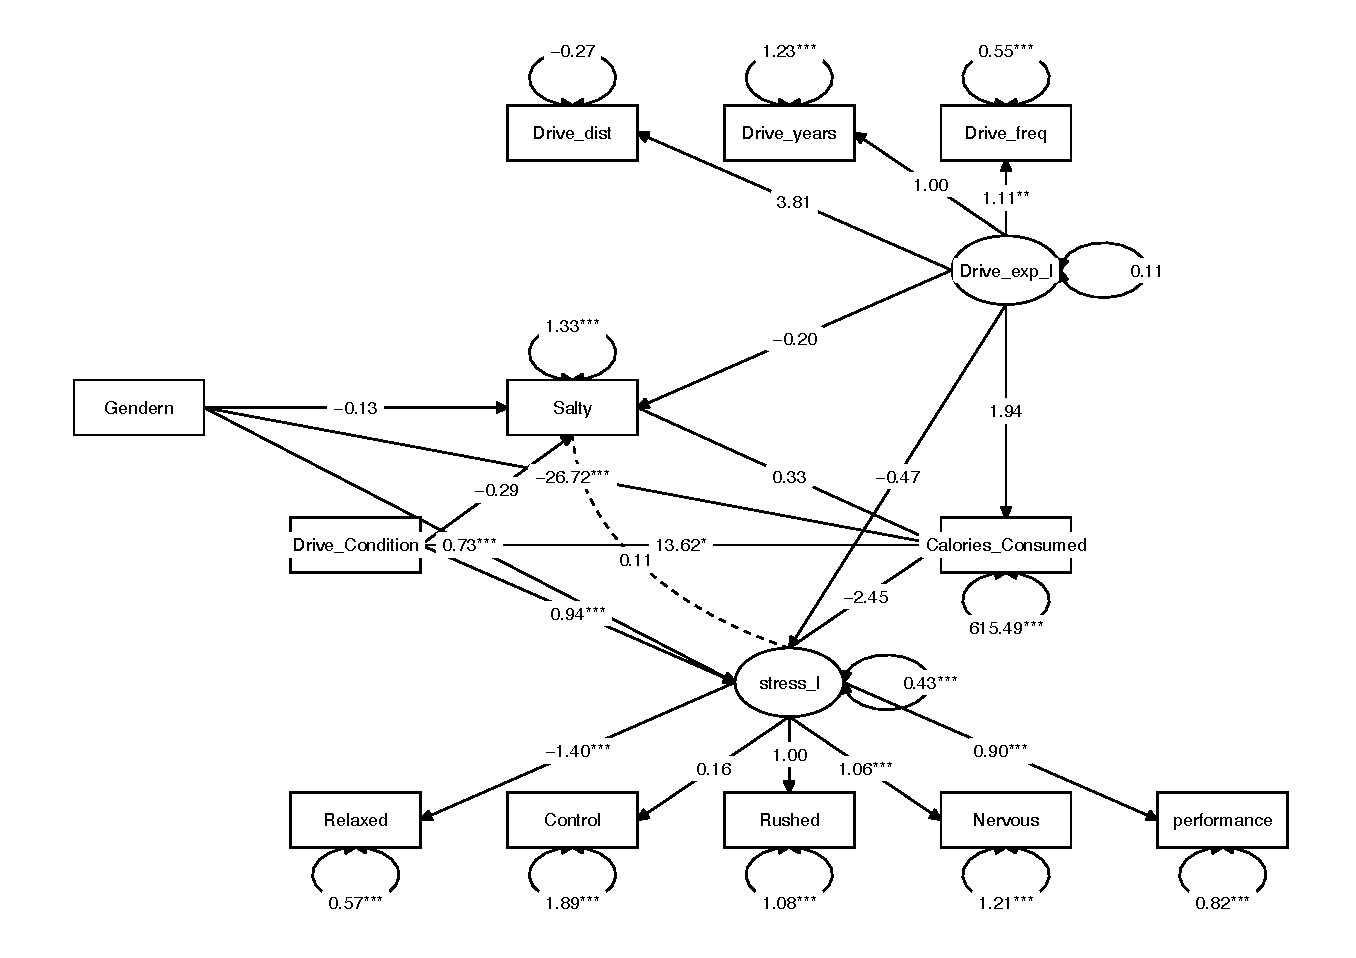
\includegraphics[width=\textwidth]{media/image6.pdf}
  \caption{Structural Equation Modeling path model. Drive\_dist = average kms driven in last year; Drive\_freq = weekly driving frequency; Drive\_years = years of having drivers’ license; Drive\_exp\_l = latent variable of driving experience; Gendern = gender, male (0) or female (1); Salty = how salty the chips were perceived during the experiment; Drive\_Condition = experimental condition, either completing a driving simulation (1) or control condition (0); Calories\_consumed = the amount of calories consumed after the driving manipulation; stress\_l = latent variable for stress experienced during the driving manipulation; Relaxed = how relaxed participants felt during the driving manipulation; Control = how in control participants felt during the driving manipulation; Rushed = how rushed participants felt during the driving manipulation; Nervous = how nervous participants felt during the driving manipulation; Performance = how well participants felt they performed during the driving manipulation.}
  \label{fig:rId28}
\end{figure}


\end{document}